\documentclass[conference]{IEEEtran}
\IEEEoverridecommandlockouts
\usepackage{cite}
\usepackage{amsmath,amssymb,amsfonts}
\usepackage{algorithmic}
\usepackage{graphicx}
\usepackage{textcomp}
\usepackage{xcolor}
\usepackage{booktabs}
\usepackage{url}
\graphicspath{{figures/}}
\def\BibTeX{{\rm B\kern-.05em{\sc i\kern-.025em b}\kern-.08em
    T\kern-.1667em\lower.7ex\hbox{E}\kern-.125emX}}
\begin{document}

\title{Echo: Zero-Shot Voice Cloning with Signal-Processing Control of Prosody}

\author{\IEEEauthorblockN{Student Name 1}
\IEEEauthorblockA{Roll No: XXXXXXXXXX \\
\textit{Dept. of Computer Science and Engineering}\\
\textit{Name of Institution}\\
City, Country \\
email@example.com}
\and
\IEEEauthorblockN{Student Name 2}
\IEEEauthorblockA{Roll No: XXXXXXXXXX \\
\textit{Dept. of Computer Science and Engineering}\\
\textit{Name of Institution}\\
City, Country \\
email@example.com}
\and
\IEEEauthorblockN{Student Name 3}
\IEEEauthorblockA{Roll No: XXXXXXXXXX \\
\textit{Dept. of Computer Science and Engineering}\\
\textit{Name of Institution}\\
City, Country \\
email@example.com}
\and
\IEEEauthorblockN{Student Name 4}
\IEEEauthorblockA{Roll No: XXXXXXXXXX \\
\textit{Dept. of Computer Science and Engineering}\\
\textit{Name of Institution}\\
City, Country \\
email@example.com}
}

\maketitle

\begin{abstract}
Modern text-to-speech models can copy the voice of a new speaker from a few seconds of audio, but
they give the user very little say over how that voice actually speaks. Echo is our attempt to
separate the two problems. A pretrained F5-TTS model produces a zero-shot clone from a five to ten
second reference clip, and everything about delivery is then handled by a prosody controller we
built ourselves using classical speech signal processing. The controller exposes eight
interpretable controls (median pitch, intonation range, contour slope, tremor, loudness, spectral
brightness, speaking rate and pause length) and combines them into six emotion presets drawn from
the vocal emotion literature. Every control is defined in a unit that can be measured back from
the output, so for each request we report what was asked for, what was actually produced and how
much speaker identity and intelligibility were lost along the way. Across four reference voices,
five test passages and thirty two conditions, the zero-shot baseline reached a speaker similarity
of 0.813 with a word error rate of 2.1 percent. Pitch requests were met to within about half a
percentage point, and even the strongest combined modification kept the word error rate unchanged
while speaker similarity fell to roughly 0.71. The system is available as a web studio and a REST
interface.
\end{abstract}

\begin{IEEEkeywords}
zero-shot voice cloning, prosody modification, PSOLA, emotional speech synthesis, speaker similarity, speech processing
\end{IEEEkeywords}

\section{Introduction}
A few years ago, cloning somebody's voice meant collecting hours of their recordings and training
or adapting a model for that one person. That is no longer the case. Recent systems such as
VALL-E~\cite{b1}, YourTTS~\cite{b2} and F5-TTS~\cite{b3} can imitate an unseen speaker from a single
short prompt, with no training at all. The speaker is defined entirely at inference time.

What these systems are less good at is letting a person decide \emph{how} the cloned voice should
sound. Prosody, meaning pitch, loudness, timing and the overall shape of intonation, is mostly
inherited from the reference clip and from whatever the model happens to sample. Some models
offer an emotion label or a speed knob, but these are learned behaviours, they are hard to inspect,
and in our early tests they did not change the output much. When we tried a built-in emotion
feature on our own voices, every setting sounded roughly the same.

Because this work was carried out for a speech processing course, we chose a different route.
Instead of asking the neural model to produce emotion, we let it do the one thing it is very good
at (copying the voice) and then reshape the delivery afterwards with signal processing that we
can explain, measure and debug. This also gives a clean experimental setup. The speaker, the text
and the backbone stay fixed, and only the prosody changes, so any loss in speaker similarity or
intelligibility can be attributed to the modification itself.

The main contributions of Echo are:
\begin{itemize}
\item a post-synthesis prosody controller with eight isolated controls, built on pitch-synchronous
overlap-add (PSOLA) resynthesis, STFT spectral shaping, gain control and pause editing, with
closed-loop correction so that the measured output matches the request;
\item six emotion presets (happy, sad, angry, calm, excited and afraid) whose parameter directions
follow published acoustic studies of vocal emotion;
\item an evaluation framework that reports control accuracy (requested versus measured) alongside
speaker similarity and word error rate, and a study of the trade-off between prosodic change and
speaker identity;
\item a working web studio and API that expose the whole pipeline.
\end{itemize}

The rest of the report is organised as follows. Section~\ref{sec:related} reviews related work.
Section~\ref{sec:system} describes the system, and Section~\ref{sec:prosody} explains the prosody
controller in detail. Section~\ref{sec:eval} covers how we measure the output, Section~\ref{sec:results}
presents the results, and Section~\ref{sec:limits} discusses limitations and ethical concerns.

\section{Related Work}\label{sec:related}

\subsection{Zero-Shot Speech Synthesis}
Early multi-speaker systems conditioned a Tacotron-style model on an embedding from a separately
trained speaker verification network~\cite{b4}. YourTTS~\cite{b2} extended this idea to VITS and
showed usable zero-shot cloning across languages. VALL-E~\cite{b1} reframed synthesis as language
modelling over neural codec tokens, using the prompt as an acoustic prefix. F5-TTS~\cite{b3}, which
we use, is a non-autoregressive model trained with flow matching~\cite{b5}. It fills in a
mel-spectrogram conditioned on the reference audio and the padded text, and a Vocos vocoder~\cite{b6}
converts the result back to a waveform. It needs no duration model or phoneme aligner, which makes it
convenient to run from a short clip and its transcript.

\subsection{Prosody Modification by Signal Processing}
Changing pitch and duration without touching the spectral envelope is an old problem. TD-PSOLA~\cite{b7}
places analysis windows at pitch marks and overlap-adds them at new spacings, which lets F0 and
timing be changed independently. Praat~\cite{b8} implements this through its Manipulation object,
which holds a pitch tier and a duration tier that can be edited and resynthesised. We access Praat
from Python through Parselmouth~\cite{b9}. For estimating a speaker-appropriate pitch range we
follow the quantile-based approach of De Looze and Hirst~\cite{b10}.

\subsection{Acoustic Correlates of Emotion}
There is a long line of work on which acoustic features signal emotion in the voice. Murray and
Arnott~\cite{b11} summarised early findings and noted that anger and joy raise pitch and widen its
range, while sadness lowers both and slows speech. Burkhardt and Sendlmeier~\cite{b12} tested
these rules with formant synthesis. Scherer~\cite{b13} and the meta-analysis by Juslin and Laukka~\cite{b14}
added voice quality and high-frequency energy to the picture, which led us to include spectral tilt
as a control. The alpha ratio we use to measure brightness comes from the eGeMAPS feature set~\cite{b15}.

\section{System Overview}\label{sec:system}

Echo is a pipeline with three stages: zero-shot synthesis, prosody control and evaluation. A FastAPI
backend runs the pipeline and a React front end, which we call the studio, lets the user record or
upload a reference, type text and adjust the controls.

\subsection{Reference Preprocessing}
The reference must be between 5 and 10 seconds long. It is converted to mono, resampled to
24~kHz (the native rate of F5-TTS and its vocoder), peak normalised and trimmed of leading and trailing
silence. We also estimate a rough signal-to-noise ratio so that the user can be warned about noisy
recordings. If no transcript is given, Whisper~\cite{b16} transcribes the reference, since F5-TTS
needs the prompt text.

\subsection{Zero-Shot Synthesis}
We use the pretrained \texttt{F5TTS\_v1\_Base} checkpoint for inference only, with 32 function
evaluations of the flow-matching solver and a fixed random seed of 42 so that runs are repeatable.
Nothing is trained or fine-tuned in this project.

One practical issue appeared early. F5-TTS tends to run consecutive sentences together, so a
multi-sentence output often had no internal pause long enough to be stretched or shortened. We
therefore split the text into sentences, synthesise each one with the same reference and seed,
trim their edges and join them with a fixed neutral gap of 0.35~s. That joined signal is the
\emph{baseline}. It is still a pure zero-shot clone, but now the pause control has something to act on.

\subsection{Prosody Control and Evaluation}
The baseline is passed to the prosody controller (Section~\ref{sec:prosody}), which returns the
\emph{controlled} signal. Both signals are then evaluated against the reference: speaker similarity,
word error rate, and a set of prosodic measurements that are compared with the requested
settings. The studio displays the two clips side by side with waveforms, mel-spectrograms, F0 and
energy contours and a table of requested versus measured values. A separate ``prosody lab'' page
applies the controller to any uploaded recording without running TTS, which was useful while
developing the DSP code.

\section{Prosody Controller}\label{sec:prosody}

\subsection{Why Pitch and Speed Were Not Enough}
Our first version only had five controls: median F0, F0 range, loudness, rate and pause length.
On paper it worked well, since the measured changes matched the requests closely. When we
listened to it, though, the emotions were hard to tell apart. A 10 percent change in F0 is less
than two semitones and a 15 percent change in RMS is around 1.2~dB, which is subtle. More
importantly, the literature~\cite{b11,b13,b14} points out that emotions differ in the \emph{shape}
of the pitch contour and in voice quality, not just in average level. Sad speech falls steadily,
happy speech is lifted, angry and joyful voices have more high-frequency energy, and fear is
often shaky. We added three controls to cover these cues and increased the preset values.

\subsection{Controls}
Table~\ref{tab:controls} lists the eight controls. Each unit was chosen so that the same quantity
can be measured from the output, which is what makes the accuracy evaluation possible.

\begin{table}[htbp]
\caption{Prosody Controls}
\begin{center}
\begin{tabular}{|l|l|c|c|}
\hline
\textbf{Control} & \textbf{Meaning (unit)} & \textbf{Neutral} & \textbf{Range} \\
\hline
Pitch & median F0 change (\%) & 0 & $-40$ to $+60$ \\
Range & F0 variation multiplier & 1.0 & 0.2 to 2.0 \\
Slope & added contour slope (st/s) & 0 & $-6$ to $+6$ \\
Tremor & 5.5~Hz F0 modulation (st) & 0 & 0 to 1.5 \\
Energy & speech RMS change (\%) & 0 & $-60$ to $+80$ \\
Brightness & spectral tilt change (dB) & 0 & $-12$ to $+12$ \\
Rate & speaking rate multiplier & 1.0 & 0.5 to 2.0 \\
Pause & internal pause multiplier & 1.0 & 0 to 3 \\
\hline
\end{tabular}
\label{tab:controls}
\end{center}
\end{table}

\subsection{Processing Chain}
The controller applies its stages in a fixed order.

\paragraph{Pauses} The signal is split into speech and silence using a threshold 35~dB below the
peak. Internal silences of at least 100~ms are stretched by inserting zeros in the middle of the gap,
or shortened by cutting out the middle. Leading and trailing silence and short closures inside
words are left alone, because editing those made consonants sound clipped.

\paragraph{Intonation and rate} All pitch and timing changes are done in a single Praat
Manipulation, so the signal is resynthesised by PSOLA only once. F0 is tracked with a
speaker-specific search range of $0.75\,Q_1$ to $2.5\,Q_3$, where $Q_1$ and $Q_3$ are the quartiles of a
first-pass estimate~\cite{b10}. The pitch tier is rewritten in semitones relative to the median
$c$ as
\begin{equation}
s'(t) = o + r\,s(t) + k\,(t - t_p) + a \sin(2\pi f_m t), \label{eq:tier}
\end{equation}
where $s(t)$ is the original contour in semitones, $o$ is the register offset from the pitch
control, $r$ is the range multiplier, $k$ is the slope in semitones per second, $t_p$ is the centre
of the current phrase, $a$ is the tremor depth and $f_m = 5.5$~Hz. Phrases are stretches of speech
separated by pauses of at least 0.1~s. The slope and tremor terms are generated in output time, so
a rate change does not alter them. The reshaped contour is soft limited beyond $\pm 8$ semitones from
the median, which kept wide-range voices out of the creaky and falsetto regions where PSOLA started
to sound rough. A constant duration tier of $1/\text{rate}$ sets the speaking rate.

\paragraph{Brightness} Spectral tilt is changed with a zero-phase STFT shelf filter that leaves
frequencies below 900~Hz untouched and applies a gain of $g$~dB above 1.1~kHz, with a smooth
transition in between. The target is the alpha ratio, the energy ratio of the 1 to 5~kHz band
to the 50~Hz to 1~kHz band~\cite{b15}. Since the effect of a given $g$ depends on the voice, the gain is
refined from the measured alpha ratio for up to three iterations. This stage also undoes the small
change in tilt that a pitch shift causes, so pitch does not leak into brightness.

\paragraph{Closed-loop correction of register and range} This was the part that took us the
longest. On real clones the open-loop mapping missed the requested median F0 by as much as 13
percent. Expanding the range or changing the spectrum alters which frames a pitch tracker treats
as voiced, so the median moves even when the target contour is correct. Our fix was to render the
full chain, measure median F0 and range exactly as the evaluation does, correct the offset and
range gain, and render again from the original signal. Rendering always starts from the original,
so PSOLA is never cascaded. At most four corrections are needed, which costs about one to two
seconds for a five second clip.

\paragraph{Energy} PSOLA and the shelf filter both change the level slightly, so after each of
these stages the speech-region RMS is restored. The requested percentage is applied last, followed
by a soft limiter with a knee at 0.85 and a ceiling at 0.99. Baselines are normalised to a peak of
0.5 so that loud presets have headroom before the limiter starts flattening them.

Thanks to these restorations the controls are isolated from each other. A pitch change does not
alter loudness or brightness, a rate change does not alter F0 or slope, and so on. Our unit tests
check this on a synthetic speech-like signal with known F0, level and pauses.

We also tried a dynamics control that expanded the loudness contrast between syllables. We removed
it in the end. Any level expander pushes the quiet edges of speech below the speech/silence
threshold, which changes the measured speech duration and pause lengths, so we could not make it
both accurate and independent of the timing controls.

\subsection{Emotion Presets}
The presets in Table~\ref{tab:presets} combine the controls following the directions reported in
\cite{b11,b12,b13}. Joy is high, wide, lifted, loud, bright and quick. Sadness is low, narrow,
falling, soft, dark and slow, with long pauses and a slight waver. Hot anger is loud, very bright
and assertively falling. Calm is slightly lowered, even and unhurried. Excitement pushes everything
up, and fear is high and fast with a clear tremor. We treat these as reasonable starting points
rather than definitions of emotion. In the studio, choosing a preset fills in the sliders, and
touching any slider switches to a custom setting.

\begin{table}[htbp]
\caption{Emotion Presets}
\begin{center}
\setlength{\tabcolsep}{3pt}
\begin{tabular}{|l|c|c|c|c|c|c|c|c|}
\hline
\textbf{Preset} & \textbf{P\%} & \textbf{Rng} & \textbf{Slp} & \textbf{Trm} & \textbf{E\%} & \textbf{Br} & \textbf{Rate} & \textbf{Pse} \\
\hline
Happy & $+15$ & 1.5 & $+1.5$ & 0 & $+20$ & $+4$ & 1.10 & 0.8 \\
Sad & $-12$ & 0.6 & $-2.5$ & 0.2 & $-30$ & $-6$ & 0.82 & 1.6 \\
Angry & $+8$ & 1.4 & $-2.0$ & 0 & $+40$ & $+8$ & 1.12 & 0.7 \\
Calm & $-6$ & 0.75 & $-1.0$ & 0 & $-15$ & $-3$ & 0.90 & 1.3 \\
Excited & $+25$ & 1.7 & $+2.0$ & 0 & $+30$ & $+5$ & 1.20 & 0.6 \\
Afraid & $+20$ & 1.2 & $+0.5$ & 0.6 & $-10$ & $+2$ & 1.18 & 0.9 \\
\hline
\multicolumn{9}{l}{P: pitch, Rng: range, Slp: slope (st/s), Trm: tremor (st),}\\
\multicolumn{9}{l}{E: energy, Br: brightness (dB), Pse: pause multiplier.}
\end{tabular}
\label{tab:presets}
\end{center}
\end{table}

\section{Evaluation Method}\label{sec:eval}

\subsection{Speaker Similarity and Intelligibility}
Speaker similarity is the cosine similarity between ECAPA-TDNN embeddings~\cite{b17} of the
reference and the generated clip, using the SpeechBrain model trained on VoxCeleb~\cite{b18}. We use it
as a relative indicator, not as a verification decision. The \emph{identity drop} of a condition
is the baseline similarity minus the similarity of the controlled clip. Intelligibility is the word
error rate between the target text and a Whisper \texttt{base.en} transcript~\cite{b16}, after
lowercasing and removing punctuation.

\subsection{Measuring Prosody}
All prosodic measurements are taken on speech regions only, after removing any DC offset. F0 is
estimated with Praat's autocorrelation tracker using a two-pass, speaker-specific range. This is a
different code path and set of parameters from the pulse analysis used for resynthesis, so the
controller cannot simply ``agree with itself''. We originally used pYIN, but on real speech it
marked noisy frames as voiced and moved the median by up to 4 percent under a pause-only edit,
which cannot change F0 at all, so we dropped it. Frames more than 7 semitones from the local
running median are treated as octave errors and folded back or discarded.

To keep the range, slope and tremor measurements from contaminating one another, the voiced
contour is decomposed in a single least-squares fit into a slow piecewise-linear intonation curve per
phrase (knots every 0.3~s), a 5.5~Hz sinusoid whose amplitude gives the tremor, and per-phrase
slopes. The range is the robust spread (interquartile range divided by 1.349) of what remains after
the tremor and slopes are removed. Energy is the speech-region RMS, brightness is the change in alpha
ratio, rate is the ratio of speech durations, and pause is the ratio of total pause time corrected
for the measured rate. For each control we report the requested value, the measured value and the
absolute error.

\subsection{Experimental Setup}
We used four reference voices taken from the demo clips bundled with F5-TTS (three distinct
recording conditions) and five fixed two-sentence passages. Each speaker and passage pair was run
under 32 conditions, giving 640 evaluated clips. The conditions were the baseline; single controls
(pitch $\pm 10$ and $\pm 20$ percent, energy $\pm 20$ percent, rate $0.8\times$ and $1.2\times$,
pause $0.5\times$ and $2\times$, range $0.6\times$ and $1.5\times$); a combined setting; the presets;
an ablation that adds controls one at a time (A: baseline, B: pitch $+15$\%, C: plus energy $+10$\%,
D: plus rate $1.1\times$, E: plus pause $1.5\times$ and range $1.2\times$); and a trade-off sweep. The
sweep moves from neutral towards a strong ``up'' target (pitch $+20$\%, range 1.5, energy $+20$\%,
rate 1.2, pause 1.5) or ``down'' target (pitch $-20$\%, range 0.6, energy $-20$\%, rate 0.8,
pause 1.5) in four levels, at 0, one third, two thirds and full strength. Everything ran on a
laptop with an RTX 4060 (8~GB) GPU under Windows 11, Python 3.12 and PyTorch 2.11. A separate
validation run covered all eight controls on two passages per speaker for every preset.

\section{Results}\label{sec:results}

\subsection{Zero-Shot Baseline}
Without any prosody control, the clones reached a mean speaker similarity of 0.813, ranging from
0.75 to 0.87 depending on the speaker, and a word error rate of 2.1 percent. With the model already
loaded on the GPU, a multi-sentence request took around 4 to 7 seconds, with the TTS stage running
at a real-time factor of about 0.8.

\subsection{Control Accuracy}
Fig.~\ref{fig:accuracy} plots measured against requested values for five controls. The points lie
close to the diagonal across the whole tested range. Pitch requests of $\pm 10$ and $\pm 20$ percent
were met to within 0.4 to 0.6 percentage points on average, energy to within 0.3 points, rate to
within 0.007 to 0.021 and pause length to within 0.04 to 0.06. The pause control was measurable
in all 20 speaker and passage pairs, which would not have been the case without sentence-level
synthesis. Intonation range is the loosest, with the spread growing at larger multipliers, mainly
because range is estimated from relatively short voiced stretches.

\begin{figure*}[htbp]
\centerline{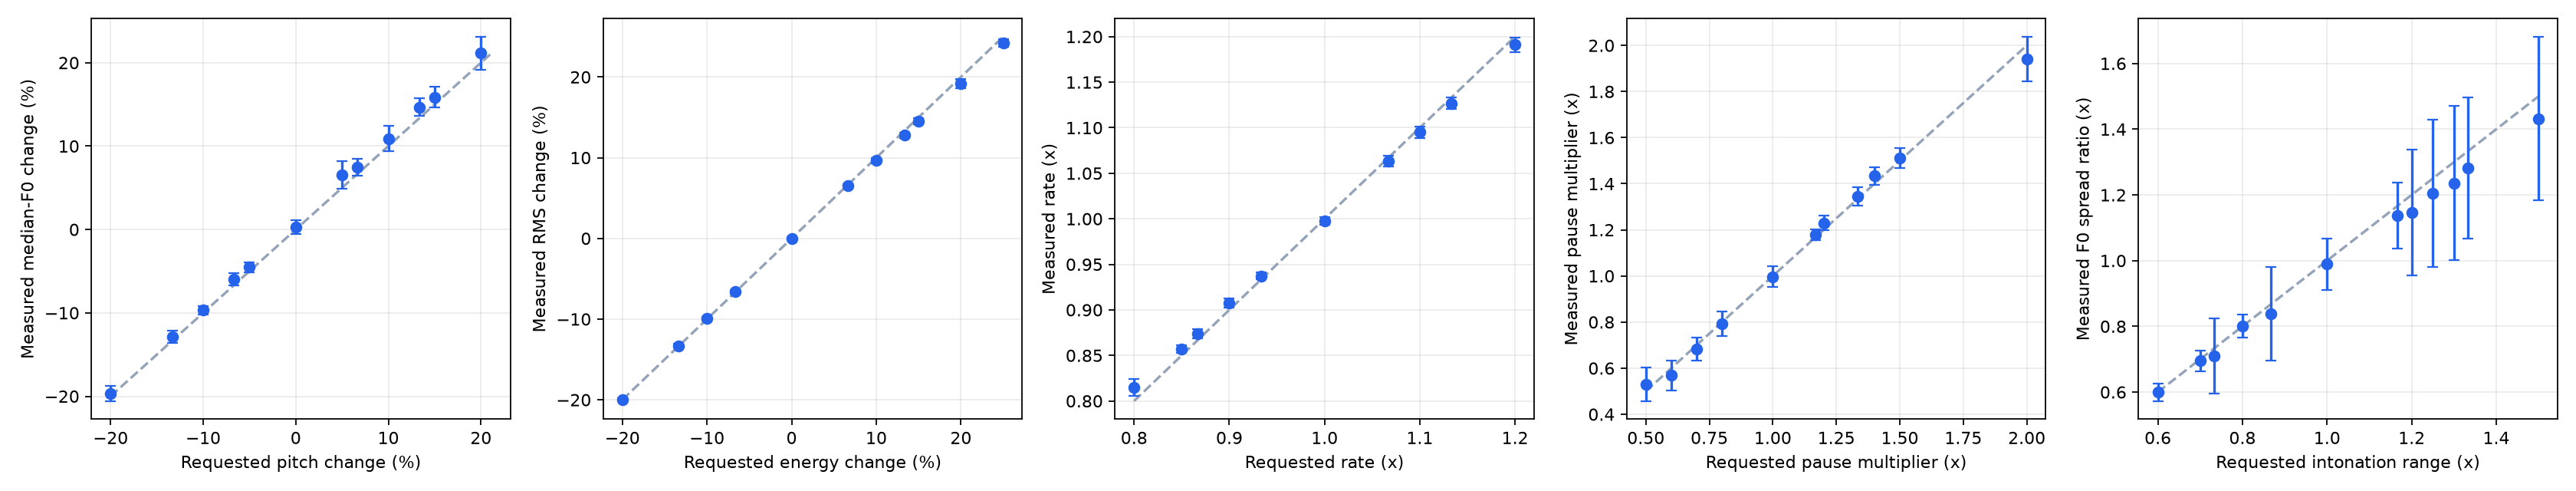
\includegraphics[width=\textwidth]{control_accuracy.png}}
\caption{Requested versus measured change for pitch, energy, rate, pause and intonation range on real
F5-TTS clones (mean and standard deviation over speakers and passages). The dashed line marks a
perfect match.}
\label{fig:accuracy}
\end{figure*}

Table~\ref{tab:validation} gives the errors from the preset validation run, which also includes
slope, tremor and brightness. Brightness, being closed loop, is almost exact. Slope and tremor show
the largest errors, but on inspection this is mostly a measurement problem rather than a control
problem. Phrases are short, and natural speech already contains 0.05 to 0.25 semitones of
micro-modulation, which makes these two quantities noisy to estimate.

\begin{table}[htbp]
\caption{Control Errors Over All Presets}
\begin{center}
\begin{tabular}{|l|c|c|}
\hline
\textbf{Control} & \textbf{Mean abs. error} & \textbf{Max abs. error} \\
\hline
Pitch & 0.33 pp & 2.8 pp \\
Range & 0.022$\times$ & 0.16$\times$ \\
Slope & 0.58 st/s & 3.2 st/s \\
Tremor & 0.14 st & 0.71 st \\
Energy & 0.23 pp & 2.1 pp \\
Brightness & 0.014 dB & 0.06 dB \\
Rate & 0.014$\times$ & 0.06$\times$ \\
Pause & 0.047$\times$ & 0.32$\times$ \\
\hline
\multicolumn{3}{l}{pp: percentage points.}
\end{tabular}
\label{tab:validation}
\end{center}
\end{table}

\subsection{Cost in Identity and Intelligibility}
Table~\ref{tab:cost} shows what each kind of change costs. The pattern is fairly clear. Pitch is
the most expensive control for speaker identity, with a $\pm 20$ percent shift lowering similarity
by about 0.09. Faster speech costs more than slower speech. Energy and pause changes are close to
free. Word error rate barely moves in any condition and stays within half a percentage point of the
baseline, so the modified speech remains just as intelligible to the recogniser.

\begin{table}[htbp]
\caption{Speaker Similarity and WER per Condition}
\begin{center}
\begin{tabular}{|l|c|c|c|}
\hline
\textbf{Condition} & \textbf{Similarity} & \textbf{Drop} & \textbf{WER} \\
\hline
Baseline & 0.813 & 0.000 & 2.1\% \\
Pitch $-20$\% & 0.723 & 0.090 & 1.7\% \\
Pitch $+20$\% & 0.725 & 0.088 & 2.1\% \\
Energy $\pm 20$\% & 0.811--0.813 & $\le$0.002 & 2.1\% \\
Rate $0.8\times$ & 0.792 & 0.021 & 1.7\% \\
Rate $1.2\times$ & 0.757 & 0.056 & 1.8\% \\
Pause $0.5\times$ / $2\times$ & 0.808 / 0.810 & $\le$0.005 & 2.1\% \\
Range $0.6\times$ / $1.5\times$ & 0.781 / 0.791 & 0.032 / 0.022 & 2.1\% \\
\hline
Ablation B (+pitch) & 0.732 & 0.081 & 2.1\% \\
Ablation D (+rate) & 0.709 & 0.104 & 2.1\% \\
Ablation E (full) & 0.724 & 0.089 & 1.7\% \\
\hline
\end{tabular}
\label{tab:cost}
\end{center}
\end{table}

The ablation tells the same story from another angle. Adding a 15 percent pitch shift accounts for
most of the identity loss on its own (0.081). Adding energy on top changes almost nothing, and
adding a 10 percent rate increase takes the drop to about 0.10. Widening the range and lengthening
pauses in the final step does not make things worse.

\subsection{Identity Versus Prosody Trade-Off}
Fig.~\ref{fig:tradeoff} shows the trade-off sweep. Speaker similarity falls steadily as the
modification gets stronger, from 0.813 at level 0 to 0.709 (up) and 0.712 (down) at level 3, which
works out to roughly 0.035 per level. The upward direction costs slightly more at the intermediate
levels. Word error rate stays flat at around 2 percent throughout. In short, prosody can be pushed a
long way without hurting what is said, and the price is paid in how much the result still sounds
like the original speaker.

\begin{figure*}[htbp]
\centerline{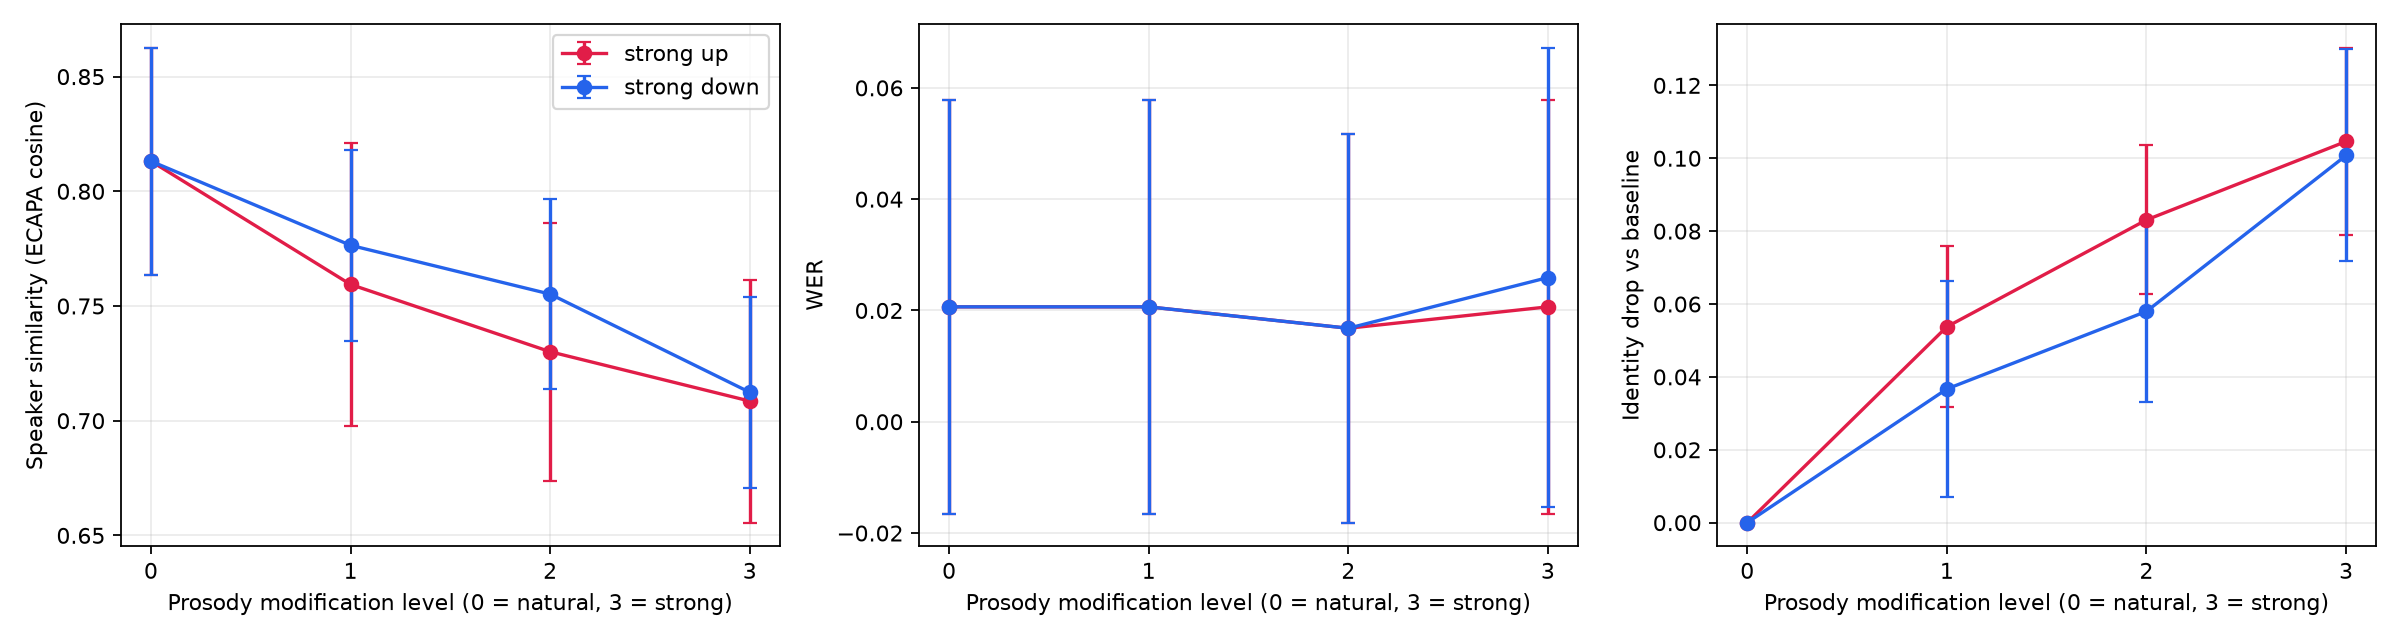
\includegraphics[width=\textwidth]{identity_prosody_tradeoff.png}}
\caption{Speaker similarity, word error rate and identity drop as the prosodic modification is
strengthened from natural (level 0) to strong (level 3), in the upward and downward directions.}
\label{fig:tradeoff}
\end{figure*}

\subsection{Presets and Perceived Emotion}
Across the presets, speaker similarity ranged from 0.79 for calm, the gentlest preset, down to
0.71 to 0.72 for excited, the most extreme one, while the word error rate stayed at or below 3
percent. To get some outside opinion on whether the presets sound emotional, we ran an
independent pretrained speech emotion recogniser (wav2vec 2.0 fine-tuned on four IEMOCAP
classes~\cite{b19}). The result was honest but modest. It labelled the unmodified clones as 72
percent neutral and kept every preset between 68 and 82 percent neutral, with only small shifts in
the expected directions; for example, excited and afraid moved towards happy, and angry gained a
little in the angry class. This is in line with older findings that rule-based prosody alone
conveys emotion only partially, since breathiness, tension and segmental detail also carry a lot
of the category. It is also known that IEMOCAP-trained classifiers do not transfer well to new
speakers and recording conditions. A proper listening test is needed before we can claim anything
about perceived emotion.

\section{Limitations and Ethics}\label{sec:limits}

\subsection{Limitations}
The study is small. Four voices with three recording conditions, one speaker encoder and no human
listening test mean the numbers should be read as indicative rather than as a benchmark.
PSOLA sounds natural for moderate edits, but shifts beyond about 30 percent and very slow rates
become audibly processed. Voice quality is limited to spectral tilt; breathiness, creak and formant
shifts such as a ``smiling'' voice are not modelled. Prosody is shaped per phrase and per utterance,
so word-level emphasis is not possible yet. Pause control depends on there being pauses to scale,
so for single-sentence text it is reported as not measurable rather than as zero error. Finally,
the F5-TTS weights are released under a non-commercial licence.

\subsection{Ethical Considerations}
Voice cloning can be misused for impersonation and fraud. Echo is meant only for recordings of
people who have agreed to have their voice cloned. Every API response and the studio interface carry
a notice that the generated speech is synthetic and must not be used to deceive anyone. Since the
pipeline runs locally, reference recordings are not sent to any outside service.

\section{Conclusion and Future Work}
Echo shows that a pretrained zero-shot cloner and a hand-built signal-processing stage make a
useful combination. The neural model takes care of the hard part, which is reproducing an unseen
voice, while the DSP controller gives precise and measurable control over pitch, contour, tremor,
loudness, brightness, rate and pauses. Because every control is defined in a measurable unit, we
could check that the output actually matched what was requested, and we found that it did so
closely, while intelligibility stayed essentially unchanged. The main cost is speaker identity, and
it comes mostly from pitch and rate changes.

There are several directions we would like to explore next. A listening test with mean opinion
scores for naturalness, similarity and perceived emotion is the most important missing piece.
Word-level emphasis could be added using the alignment between text and audio. Modelling
breathiness and formant changes would widen the range of voice qualities. It would also be
interesting to use the controller's measurements as targets for a lightweight learned model, which
might reduce the identity cost of large pitch shifts.

\section*{Acknowledgment}
We thank our course instructor for the guidance given throughout this project. We also thank the
authors of F5-TTS, SpeechBrain, Whisper, Praat and Parselmouth for releasing their work openly,
which made this project possible.

\begin{thebibliography}{00}
\bibitem{b1} C. Wang, S. Chen, Y. Wu, Z. Zhang, L. Zhou, S. Liu, Z. Chen, Y. Liu, H. Wang, J. Li, L. He, S. Zhao, and F. Wei, ``Neural codec language models are zero-shot text to speech synthesizers,'' arXiv:2301.02111, 2023.
\bibitem{b2} E. Casanova, J. Weber, C. Shulby, A. C. Junior, E. G\"olge, and M. A. Ponti, ``YourTTS: Towards zero-shot multi-speaker TTS and zero-shot voice conversion for everyone,'' in Proc. ICML, 2022, pp. 2709--2720.
\bibitem{b3} Y. Chen, Z. Niu, Z. Ma, K. Deng, C. Wang, J. Zhao, K. Yu, and X. Chen, ``F5-TTS: A fairytaler that fakes fluent and faithful speech with flow matching,'' arXiv:2410.06885, 2024.
\bibitem{b4} Y. Jia, Y. Zhang, R. J. Weiss, Q. Wang, J. Shen, F. Ren, Z. Chen, P. Nguyen, R. Pang, I. Lopez Moreno, and Y. Wu, ``Transfer learning from speaker verification to multispeaker text-to-speech synthesis,'' in Proc. NeurIPS, 2018.
\bibitem{b5} Y. Lipman, R. T. Q. Chen, H. Ben-Hamu, M. Nickel, and M. Le, ``Flow matching for generative modeling,'' in Proc. ICLR, 2023.
\bibitem{b6} H. Siuzdak, ``Vocos: Closing the gap between time-domain and Fourier-based neural vocoders for high-quality audio synthesis,'' arXiv:2306.00434, 2023.
\bibitem{b7} E. Moulines and F. Charpentier, ``Pitch-synchronous waveform processing techniques for text-to-speech synthesis using diphones,'' Speech Communication, vol. 9, no. 5--6, pp. 453--467, 1990.
\bibitem{b8} P. Boersma and D. Weenink, ``Praat: doing phonetics by computer,'' computer program, \url{http://www.praat.org/}.
\bibitem{b9} Y. Jadoul, B. Thompson, and B. de Boer, ``Introducing Parselmouth: A Python interface to Praat,'' Journal of Phonetics, vol. 71, pp. 1--15, 2018.
\bibitem{b10} C. De Looze and D. Hirst, ``Detecting changes in key and range for the automatic modelling and coding of intonation,'' in Proc. Speech Prosody, 2008, pp. 135--138.
\bibitem{b11} I. R. Murray and J. L. Arnott, ``Toward the simulation of emotion in synthetic speech: A review of the literature on human vocal emotion,'' J. Acoust. Soc. Am., vol. 93, no. 2, pp. 1097--1108, 1993.
\bibitem{b12} F. Burkhardt and W. F. Sendlmeier, ``Verification of acoustical correlates of emotional speech using formant-synthesis,'' in Proc. ISCA Workshop on Speech and Emotion, 2000, pp. 151--156.
\bibitem{b13} K. R. Scherer, ``Vocal communication of emotion: A review of research paradigms,'' Speech Communication, vol. 40, no. 1--2, pp. 227--256, 2003.
\bibitem{b14} P. N. Juslin and P. Laukka, ``Communication of emotions in vocal expression and music performance: Different channels, same code?'' Psychological Bulletin, vol. 129, no. 5, pp. 770--814, 2003.
\bibitem{b15} F. Eyben, K. R. Scherer, B. W. Schuller, J. Sundberg, E. Andr\'e, C. Busso, L. Y. Devillers, J. Epps, P. Laukka, S. S. Narayanan, and K. P. Truong, ``The Geneva minimalistic acoustic parameter set (GeMAPS) for voice research and affective computing,'' IEEE Trans. Affective Computing, vol. 7, no. 2, pp. 190--202, 2016.
\bibitem{b16} A. Radford, J. W. Kim, T. Xu, G. Brockman, C. McLeavey, and I. Sutskever, ``Robust speech recognition via large-scale weak supervision,'' in Proc. ICML, 2023, pp. 28492--28518.
\bibitem{b17} B. Desplanques, J. Thienpondt, and K. Demuynck, ``ECAPA-TDNN: Emphasized channel attention, propagation and aggregation in TDNN based speaker verification,'' in Proc. Interspeech, 2020, pp. 3830--3834.
\bibitem{b18} M. Ravanelli \textit{et al.}, ``SpeechBrain: A general-purpose speech toolkit,'' arXiv:2106.04624, 2021.
\bibitem{b19} C. Busso, M. Bulut, C.-C. Lee, A. Kazemzadeh, E. Mower, S. Kim, J. N. Chang, S. Lee, and S. S. Narayanan, ``IEMOCAP: Interactive emotional dyadic motion capture database,'' Language Resources and Evaluation, vol. 42, no. 4, pp. 335--359, 2008.
\end{thebibliography}

\end{document}
